
\section{Struttura Fisica del Sistema di HBS}

In figura~\ref{fig:physical-view} viene illustrata la struttura fisica del sistema di HBS.
In nodi in figura rappresentano \emph{macchine fisiche} su cui il software di HBS viene eseguito.

\begin{figure*}[h]
	\centering
	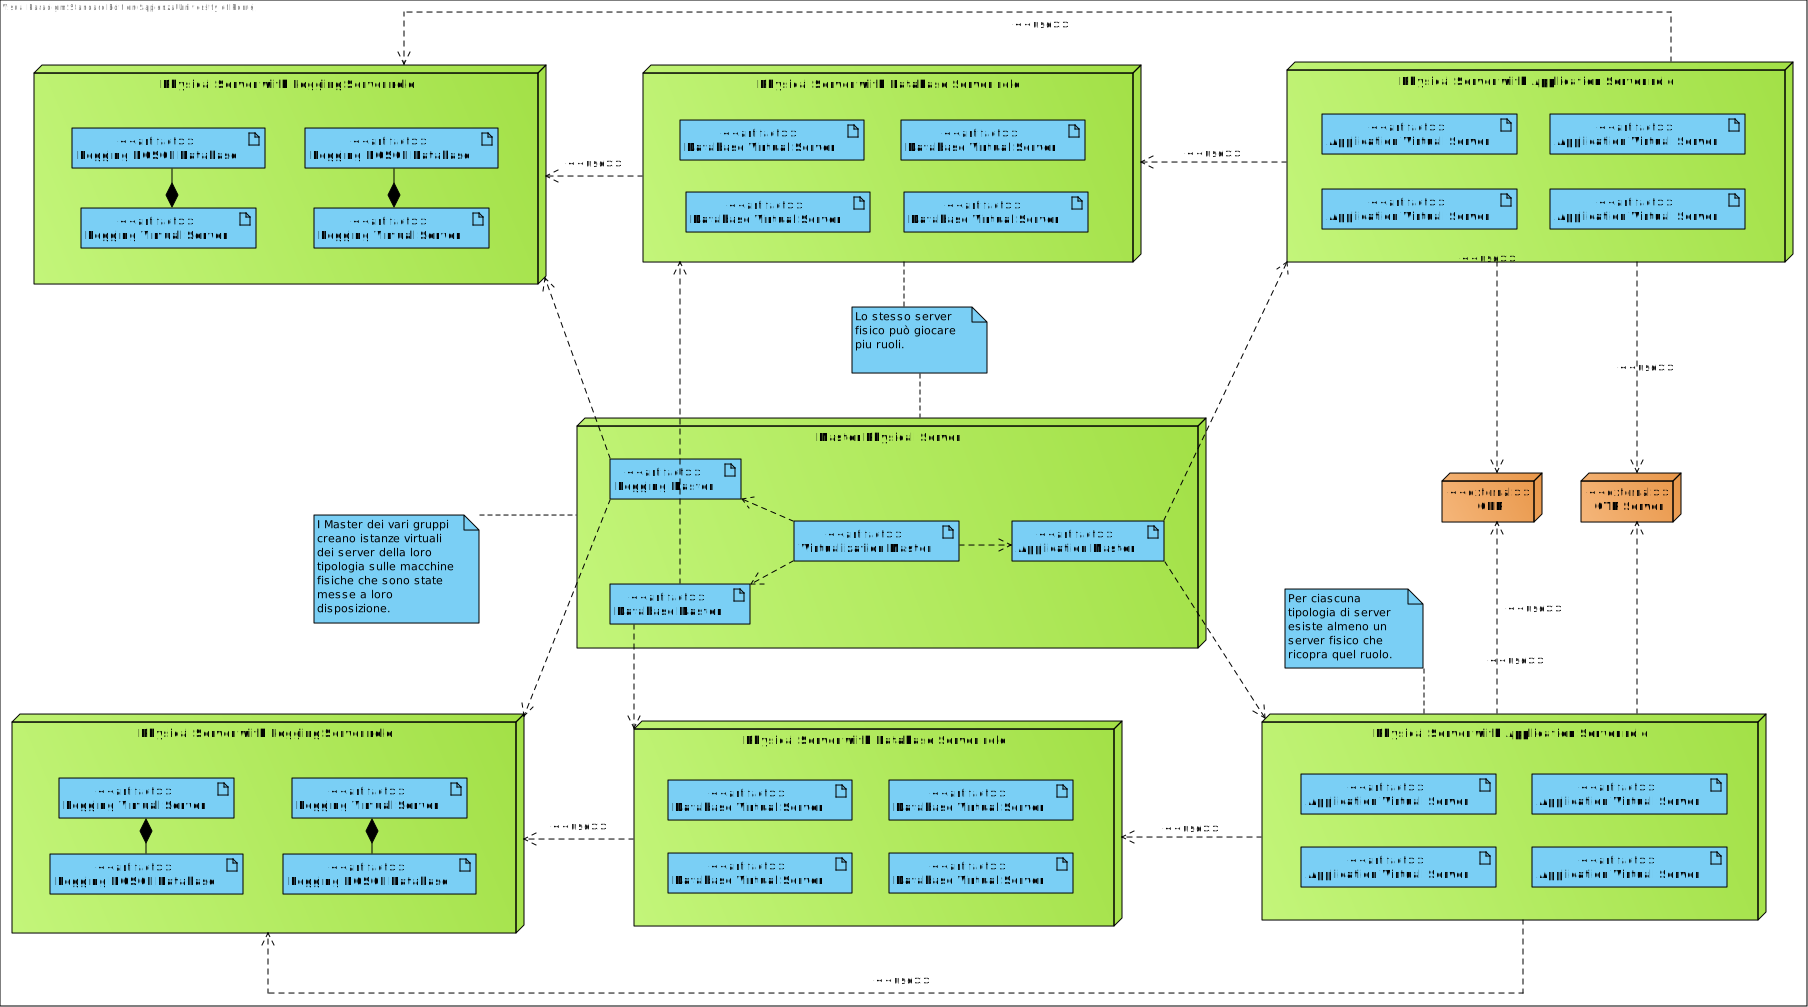
\includegraphics[width=\textheight, angle=90]{Images/Physical_View.eps}
	\caption{Diagramma di deployment del sistema.}
	\label{fig:physical-view}
\end{figure*}

I ruoli comprendono:
\begin{description}
	\item[Database Server] macchina abilitata all'esecuzione di istanze del database di HBS;

	\item[Application Server] macchina abilitata all'esecuzione di istanze dell'applicazione principale di HBS;

	\item[Logging Server] macchina abilitata all'esecuzione di istanze del sistema di logging.
\end{description}
Ciascuna macchina pu\`o ricoprire diversi ruoli.

Una macchina nel sistema ricopre il ruolo di \emph{master}.
Su questa macchina sono in esecuzione i processi di gestione delle istanze del database, dell'applicazione principale, e dei sistemi di logging.
I processi di gestione dei sotto-sistemi si occupano di avviare istanze virtuali dei propri sotto-sistemi sulle macchine messe a disposizione dal \emph{virtualization master}.
